% You should title the file with a .tex extension (hw1.tex, for example)
\documentclass[a4paper, 11pt]{article}

\usepackage{amsmath}
\usepackage{amssymb}
\usepackage{fancyhdr}
\usepackage{graphicx}
\usepackage{scribe}
\usepackage{tikz}
\usepackage{graphicx}
\usepackage[margin=1in]{geometry}
\usepackage{graphicx}
\newcommand{\question}[2] {\vspace{.25in} \hrule\vspace{0.5em}
\noindent{\bf #1: #2} \vspace{0.5em}
\hrule \vspace{.10in}}
\renewcommand{\part}[1] {\vspace{.10in} {\bf (#1)}}

\newcommand{\myname}{Kriangsak Thuiprakhon}
\newcommand{\myemail}{kriangsak.thi@student.mahidol.edu}
\newcommand{\myhwnum}{2}

\setlength{\parindent}{0pt}
\setlength{\parskip}{5pt plus 1pt}
 


\begin{document}

\medskip                        % Skip a "medium" amount of space
                                % (latex determines what medium is)
                                % Also try: \bigskip, \littleskip

\thispagestyle{plain}
\begin{center}                  % Center the following lines
{\Large ICCS240: Assignment \myhwnum} \\
\myname \\
\myemail \\
Collaborator: {Prof and 1409 ppl}
\end{center}
\question{2}{Relational Database Design Theory}
\part{1} Alice \textit{vs} Bob
Given 
\begin{verbatim}
Contracts( c_no, supp_no, proj_no, dept_no, part_no, qty, val)
\end{verbatim}
Let  $\mathcal{F}_A$ and $\mathcal{F}_B$  denote the set of functional dependencies  of Alice and Bob respectively. Here, for simplicity, we rewrite the relation to be
\begin{verbatim}
 Contracts( C, S Pr, D, Pa, Q, V) \end{verbatim} then.\\
 \begin{align*}
\mathcal{F}_A &= \{ &&C \rightarrow SPrDPaQV, \quad &PrPa \rightarrow C, \quad &&&SD \rightarrow Pa \} \\
\mathcal{F}_B &= \{ &&C \rightarrow SPrD, \quad &PrPa \rightarrow C, \quad &&&SDPr \rightarrow CPaQV \} 
 \end{align*}
As per Bob's schema, it was designed such that for $Pa$ to be determined, it needs $SDPr$ altogether to do so, meanwhile, in Alice's, only $SD$ can determine Pa. Therefore, the two designs are different.

\part{2} Given three disjoint ordered sets of attributes $ \alpha, \beta, \gamma $, consider relations $R=(\alpha, \beta, \gamma)$ and its decomposition: $R_1 = (\alpha, \beta) $and $R_2 =( \alpha,  \gamma)$.That is, $R_1 = \Pi_{R_1}(R)$ and $R_2 = \Pi_{R_2}(R)$. Assume  $R_1 \cap R_2 \rightarrow R_1$, that is ($\alpha \rightarrow \alpha \beta$). Prove/disprove that 
\begin{claim}
$$
R = R_1 \bowtie R_2
$$
\end{claim}

\begin{proof}
Let's take a look at RHS, as discussed in class that Natural join is a derived operation that can be expressed as:

Let
\begin{itemize}
\item   Each of the attribute sets have $m$ elements

\item  $A$ denote the set of attributes in $R_1$ 

\item $B$ denote the set of attributes in $R_2$ 
\end{itemize}
\begin{align}
R_1 \bowtie R_2 &= \Pi_{A \cup B} ( \sigma_{\alpha = \varepsilon} (\rho_{\alpha \rightarrow \varepsilon} (R_1) \times R_2)))\\
&=  \Pi_{A \cup B} ( \sigma_{\alpha = \varepsilon} (\{ \left (\alpha_i,\beta_i,\varepsilon_j,\gamma_j) \quad \forall i,j =\{1,2,3,\cdots m\} \right \})) \\
&= \Pi_{A \cup B} ( \{ \left (\alpha_i,\beta_i,\varepsilon_j,\gamma_j) \quad | \quad \alpha_i = \varepsilon_j  \right )\}) \\
&= \Pi_{A \cup B} ( F(\alpha^*,\beta^*,\varepsilon^*,\gamma^*)) &\textmd{ For some relation }F\\
&= \Pi_{A \cup B} ( F(\alpha^*,\beta^*,\varepsilon^*,\gamma^*)) \\ 
&= F(\alpha^*,\beta^*,\gamma^*) \\
\end{align}
From here on,
%Since  the two relations have exactly the same set of attributes with the same set of elements, from the select condition, relation $R=F$. 
we now need to show that the relations $R$ and $F$ are equal. 
\begin{claim}
 Relation $R$ is  equal to resulting relation $F$ in $(7)$. That is,
 $$
 R(\alpha,\beta ,\gamma) = F (\alpha^*,\beta^* ,\gamma^*) \Leftrightarrow  (\alpha,\beta ,\gamma) = (\alpha^*,\beta^* ,\gamma^*)
 $$
\end{claim}
\begin{proof}
From above, line (3), it is clear that each remaining pair of tuples was compared only by the value of $\alpha$, such that  $ \alpha_i = \varepsilon_j $. This will happen if  and only if $i=j$. This implies that  $(\alpha,\beta ,\gamma) = (\alpha^*,\beta^* ,\gamma^*)$
\end{proof}
From \textit{claim 0.2}, it is shown that  relations$ R_1 \bowtie R_2 = R $. Hence proved.
\end{proof}

\part{3} Consider relation $R(A,B,C,D)$,with $\mathcal{F} = \{ AB \rightarrow C, \quad BC \rightarrow D, \quad CD \rightarrow A \} $
\begin{itemize}
	\item Is R in BCNF? 
	
	To answer this question, we first need to identify the candidate keys. The candidate keys in this relation  are $  AB, BC$ since  $ AB^+, BC^+ = \{ A,B,C,D \}$ Now we can tell that this relation is not in $BCNF$ since it is \textit{not} the case that  \textit{ every} determinant is a superkey.\
	\item Decompose the  $R(A,B,C,D)$ into $R_1(B,C,D)$ and $R_2(C,D,A)$. Let us consider each decomposed relations at a time.
	\begin{itemize}
	\item[(i)] For $R_1(B,C,D)$ We can now determine the new set of functional dependency. That is, we will only take the subset of $\mathcal{F}$ that $R_1$ is relevant to. Then,
	$$\mathcal{F}_{R_1} = \{BC \rightarrow D \}$$ 
	\item[(ii)] For $R_2(C,D,A)$
	$$\mathcal{F}_{R_2} = \{CD \rightarrow A \}$$ 
\end{itemize}	 
Now, the two relations are of BCNF since each of them satisfies the condition:  \textit{ every} determinant is a superkey.
\item The decomposition is lossless if at least one of the following functional
dependencies are in $\mathcal{F}^+$ (closure of every attribute or attribute sets in  $\mathcal{F}$). 
\begin{itemize}
\item[(i)] $R_1 \cap R_2 \rightarrow R_1$. Apply our relations,
$$
R_1 \cap R_2 = AC \rightarrow ABC
$$
\item[(ii)] 
$R_1 \cap R_2 \rightarrow R_2$Apply our relations,
$$
R_1 \cap R_2 = AC \rightarrow ACD
$$
\end{itemize}
From the given $\mathcal{F}$, the closure of attributes are as follows:
\begin{align*}
AB^+ &= \{A, B,C,D \}\\
BC^+ &= \{A,B,C,D \}\\
CD^+ &=\{C,D,A\}
\end{align*} 
We can now see that there is  neither $AC \rightarrow ABC$ nor $AC \rightarrow ACD$ belongs to $\mathcal{F}$, hence, the decomposition is not lossless. 
\clearpage

\item Relation $R$ is of 3NF if at least one of the following requirements is met:\\
For any $X \rightarrow Z$ in $\mathcal{F}$
\begin{itemize}
\item[(i)] $X$ is \textit{not a superkey}
\item[(ii)] $A$ is not \textit{prime} 
\end{itemize}
Since $CD \rightarrow A $ only violates the \textit{(ii)}, the relation R is of \textbf{3NF}
\end{itemize}

\question{3}{Storage and Indexing} 
\part{1}  which would most likely require the fewest I/Os for processing the query.\\
\begin{itemize}
\item scanning through the whole heap file for R since what is needed is the tuple of the relation R, doing so will take $O(n)$.
\item Use B+ tree, this is done in the similar fashion of Binary Search. From Data Structure, BST, takes at most $O( \log_{\frac{k}{2}} n ) $ \textit{w.h.p.}
\item Use Hash Index, this takes amortized $O(1)$.
\end{itemize}
\part{2} 
\begin{itemize}
\item B+  tree with this exact order of insertion: 10, 20, 30, 40, 50, 60, 70, 80, 90, 100.
The tree will be built based on the following property:
\begin{itemize}
\item oder(k) = 3
\item pointer(k+1) = 4
\item minKey (k/2) = 3/2 = 1:
\item maxKey (k-1) = 2 



\tikzset{every picture/.style={line width=0.75pt}} %set default line width to 0.75pt        

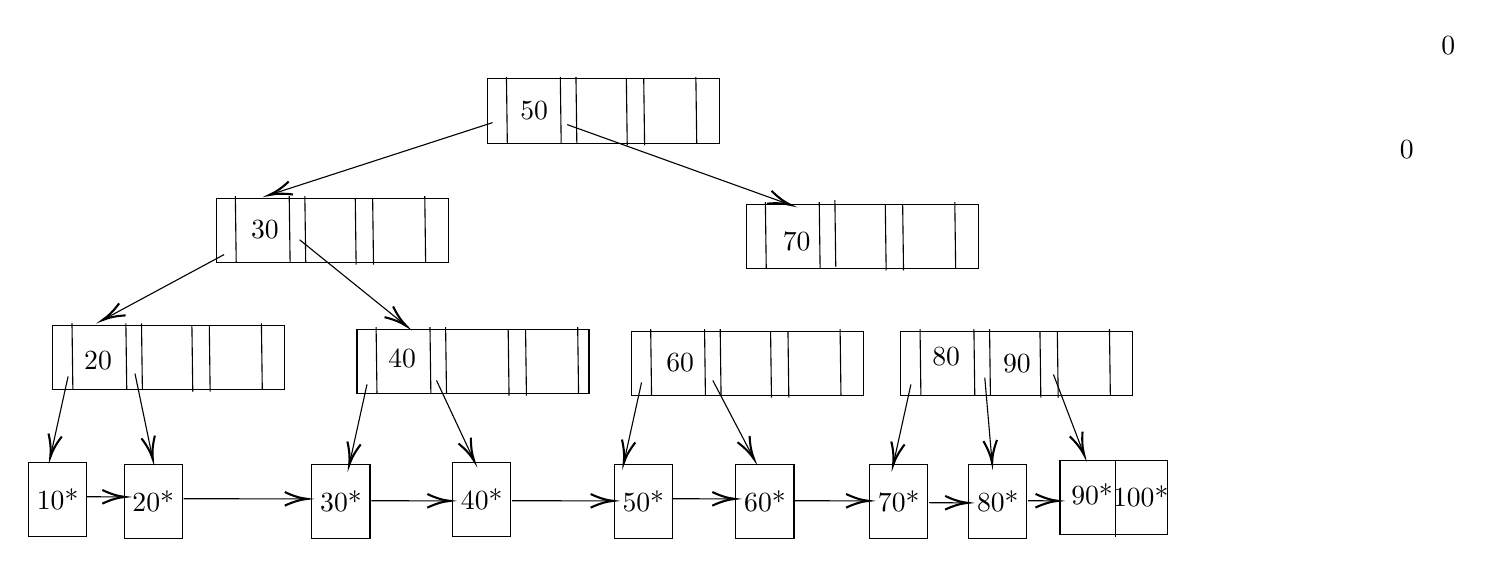
\begin{tikzpicture}[x=0.75pt,y=0.75pt,yscale=-1,xscale=1]
%uncomment if require: \path (0,345); %set diagram left start at 0, and has height of 345

%Shape: Rectangle [id:dp32574316465336217] 
\draw   (258.04,36.96) -- (369.81,36.96) -- (369.81,68) -- (258.04,68) -- cycle ;
%Straight Lines [id:da26653663223388] 
\draw    (293.2,36) -- (293.62,68) ;
%Straight Lines [id:da7385090454691864] 
\draw    (300.74,36) -- (301.16,68) ;
%Straight Lines [id:da8544299118360646] 
\draw    (267.25,36) -- (267.67,68) ;
%Straight Lines [id:da930732509680896] 
\draw    (325.02,36.96) -- (325.44,68.96) ;
%Straight Lines [id:da69512074796696] 
\draw    (333.39,36.96) -- (333.81,68.96) ;
%Straight Lines [id:da11381375915778624] 
\draw    (358.51,36) -- (358.93,68) ;
%Shape: Rectangle [id:dp5564235763237072] 
\draw   (127.42,94.38) -- (239.2,94.38) -- (239.2,125.42) -- (127.42,125.42) -- cycle ;
%Straight Lines [id:da102373038106776] 
\draw    (162.59,93.42) -- (163.01,125.42) ;
%Straight Lines [id:da5333943980458339] 
\draw    (170.12,93.42) -- (170.54,125.42) ;
%Straight Lines [id:da4097691419968579] 
\draw    (136.63,93.42) -- (137.05,125.42) ;
%Straight Lines [id:da3996471452585759] 
\draw    (194.41,94.38) -- (194.82,126.37) ;
%Straight Lines [id:da011032150201289226] 
\draw    (202.78,94.38) -- (203.2,126.37) ;
%Straight Lines [id:da802407879380034] 
\draw    (227.9,93.42) -- (228.31,125.42) ;
%Shape: Rectangle [id:dp9979129201079927] 
\draw   (382.79,97.25) -- (494.56,97.25) -- (494.56,128.29) -- (382.79,128.29) -- cycle ;
%Straight Lines [id:da16625765432954998] 
\draw    (417.95,96.29) -- (418.37,128.29) ;
%Straight Lines [id:da3647031842982146] 
\draw    (425.49,95.33) -- (425.91,127.33) ;
%Straight Lines [id:da8115786020974805] 
\draw    (392,96.29) -- (392.42,128.29) ;
%Straight Lines [id:da5222139177284297] 
\draw    (449.77,97.25) -- (450.19,129.25) ;
%Straight Lines [id:da24030239615721194] 
\draw    (458.14,97.25) -- (458.56,129.25) ;
%Straight Lines [id:da21971037892600864] 
\draw    (483.26,96.29) -- (483.68,128.29) ;
%Shape: Rectangle [id:dp13852793009269737] 
\draw   (48.72,155.62) -- (160.5,155.62) -- (160.5,186.66) -- (48.72,186.66) -- cycle ;
%Straight Lines [id:da5103414588651092] 
\draw    (83.89,154.67) -- (84.31,186.66) ;
%Straight Lines [id:da8712020319990447] 
\draw    (91.42,154.67) -- (91.84,186.66) ;
%Straight Lines [id:da8558156170331271] 
\draw    (57.93,154.67) -- (58.35,186.66) ;
%Straight Lines [id:da15205331219254947] 
\draw    (115.7,155.62) -- (116.12,187.62) ;
%Straight Lines [id:da5129923547556717] 
\draw    (124.08,155.62) -- (124.49,187.62) ;
%Straight Lines [id:da7712823745198085] 
\draw    (149.19,154.67) -- (149.61,186.66) ;
%Shape: Rectangle [id:dp13870733259165058] 
\draw   (195.24,157.54) -- (307.02,157.54) -- (307.02,188.58) -- (195.24,188.58) -- cycle ;
%Straight Lines [id:da005178574681245163] 
\draw    (230.41,156.58) -- (230.83,188.58) ;
%Straight Lines [id:da309869691513728] 
\draw    (237.94,156.58) -- (238.36,188.58) ;
%Straight Lines [id:da21093730736466232] 
\draw    (204.45,156.58) -- (204.87,188.58) ;
%Straight Lines [id:da7805076775703609] 
\draw    (268.08,157.54) -- (268.5,189.54) ;
%Straight Lines [id:da5943458847962444] 
\draw    (276.46,157.54) -- (276.88,189.54) ;
%Straight Lines [id:da2705615797915406] 
\draw    (301.57,156.58) -- (301.99,188.58) ;
%Shape: Rectangle [id:dp6253699450090605] 
\draw   (327.53,158.49) -- (439.3,158.49) -- (439.3,189.54) -- (327.53,189.54) -- cycle ;
%Straight Lines [id:da3239451920625164] 
\draw    (362.7,157.54) -- (363.11,189.54) ;
%Straight Lines [id:da7368468636615368] 
\draw    (370.23,157.54) -- (370.65,189.54) ;
%Straight Lines [id:da35508729261256355] 
\draw    (336.74,157.54) -- (337.16,189.54) ;
%Straight Lines [id:da1282301661816645] 
\draw    (394.51,158.49) -- (394.93,190.49) ;
%Straight Lines [id:da6284444300247394] 
\draw    (402.88,158.49) -- (403.3,190.49) ;
%Straight Lines [id:da7908326003834188] 
\draw    (428,157.54) -- (428.42,189.54) ;
%Shape: Rectangle [id:dp6137515015342755] 
\draw   (457.31,158.49) -- (569.08,158.49) -- (569.08,189.54) -- (457.31,189.54) -- cycle ;
%Straight Lines [id:da5137355792125323] 
\draw    (492.47,157.54) -- (492.89,189.54) ;
%Straight Lines [id:da6413034625859316] 
\draw    (500.01,157.54) -- (500.42,189.54) ;
%Straight Lines [id:da3272426529932686] 
\draw    (466.52,157.54) -- (466.93,189.54) ;
%Straight Lines [id:da5406616881295853] 
\draw    (524.29,158.49) -- (524.71,190.49) ;
%Straight Lines [id:da5906079850634157] 
\draw    (532.66,158.49) -- (533.08,190.49) ;
%Straight Lines [id:da07269456922064865] 
\draw    (557.78,157.54) -- (558.2,189.54) ;
%Shape: Rectangle [id:dp7459564918205305] 
\draw   (37,221.65) -- (65.05,221.65) -- (65.05,257.48) -- (37,257.48) -- cycle ;
%Shape: Rectangle [id:dp9844375392143719] 
\draw   (83.05,222.61) -- (111.1,222.61) -- (111.1,258.44) -- (83.05,258.44) -- cycle ;
%Shape: Rectangle [id:dp360895120622042] 
\draw   (173.47,222.61) -- (201.52,222.61) -- (201.52,258.44) -- (173.47,258.44) -- cycle ;
%Shape: Rectangle [id:dp8898273177006085] 
\draw   (241.29,221.65) -- (269.34,221.65) -- (269.34,257.48) -- (241.29,257.48) -- cycle ;
%Shape: Rectangle [id:dp29186889678913963] 
\draw   (319.16,222.61) -- (347.21,222.61) -- (347.21,258.44) -- (319.16,258.44) -- cycle ;
%Shape: Rectangle [id:dp4648355798217013] 
\draw   (377.77,222.61) -- (405.81,222.61) -- (405.81,258.44) -- (377.77,258.44) -- cycle ;
%Shape: Rectangle [id:dp9051210316339248] 
\draw   (442.23,222.61) -- (470.28,222.61) -- (470.28,258.44) -- (442.23,258.44) -- cycle ;
%Shape: Rectangle [id:dp5927846473939024] 
\draw   (489.96,222.61) -- (518.01,222.61) -- (518.01,258.44) -- (489.96,258.44) -- cycle ;
%Shape: Rectangle [id:dp7048816497562429] 
\draw   (533.92,220.7) -- (585.83,220.7) -- (585.83,256.52) -- (533.92,256.52) -- cycle ;
%Straight Lines [id:da3801513815190848] 
\draw    (560.71,221.12) -- (560.71,257.48) ;
%Straight Lines [id:da966696285693353] 
\draw    (260.55,58.01) -- (154.86,92.26) ;
\draw [shift={(152.96,92.88)}, rotate = 342.03999999999996] [color={rgb, 255:red, 0; green, 0; blue, 0 }  ][line width=0.75]    (10.93,-3.29) .. controls (6.95,-1.4) and (3.31,-0.3) .. (0,0) .. controls (3.31,0.3) and (6.95,1.4) .. (10.93,3.29)   ;
%Straight Lines [id:da5778572638983835] 
\draw    (296.55,58.97) -- (402.26,96.99) ;
\draw [shift={(404.14,97.67)}, rotate = 199.78] [color={rgb, 255:red, 0; green, 0; blue, 0 }  ][line width=0.75]    (10.93,-3.29) .. controls (6.95,-1.4) and (3.31,-0.3) .. (0,0) .. controls (3.31,0.3) and (6.95,1.4) .. (10.93,3.29)   ;
%Straight Lines [id:da6373025984910785] 
\draw    (131.19,121.59) -- (74.34,152.22) ;
\draw [shift={(72.58,153.17)}, rotate = 331.68] [color={rgb, 255:red, 0; green, 0; blue, 0 }  ][line width=0.75]    (10.93,-3.29) .. controls (6.95,-1.4) and (3.31,-0.3) .. (0,0) .. controls (3.31,0.3) and (6.95,1.4) .. (10.93,3.29)   ;
%Straight Lines [id:da5921462612949191] 
\draw    (167.61,114.47) -- (217.55,154.78) ;
\draw [shift={(219.1,156.04)}, rotate = 218.91] [color={rgb, 255:red, 0; green, 0; blue, 0 }  ][line width=0.75]    (10.93,-3.29) .. controls (6.95,-1.4) and (3.31,-0.3) .. (0,0) .. controls (3.31,0.3) and (6.95,1.4) .. (10.93,3.29)   ;
%Straight Lines [id:da6652078600110307] 
\draw    (56.05,180.29) -- (47.9,217.25) ;
\draw [shift={(47.47,219.2)}, rotate = 282.44] [color={rgb, 255:red, 0; green, 0; blue, 0 }  ][line width=0.75]    (10.93,-3.29) .. controls (6.95,-1.4) and (3.31,-0.3) .. (0,0) .. controls (3.31,0.3) and (6.95,1.4) .. (10.93,3.29)   ;
%Straight Lines [id:da9377274940197003] 
\draw    (88.28,178.92) -- (96.46,218.2) ;
\draw [shift={(96.86,220.16)}, rotate = 258.24] [color={rgb, 255:red, 0; green, 0; blue, 0 }  ][line width=0.75]    (10.93,-3.29) .. controls (6.95,-1.4) and (3.31,-0.3) .. (0,0) .. controls (3.31,0.3) and (6.95,1.4) .. (10.93,3.29)   ;
%Straight Lines [id:da34383806266901884] 
\draw    (200.06,184.12) -- (191.91,221.08) ;
\draw [shift={(191.47,223.03)}, rotate = 282.44] [color={rgb, 255:red, 0; green, 0; blue, 0 }  ][line width=0.75]    (10.93,-3.29) .. controls (6.95,-1.4) and (3.31,-0.3) .. (0,0) .. controls (3.31,0.3) and (6.95,1.4) .. (10.93,3.29)   ;
%Straight Lines [id:da4084711993238651] 
\draw    (233.55,182.21) -- (250.91,219.3) ;
\draw [shift={(251.76,221.12)}, rotate = 244.92000000000002] [color={rgb, 255:red, 0; green, 0; blue, 0 }  ][line width=0.75]    (10.93,-3.29) .. controls (6.95,-1.4) and (3.31,-0.3) .. (0,0) .. controls (3.31,0.3) and (6.95,1.4) .. (10.93,3.29)   ;
%Straight Lines [id:da5677294616478823] 
\draw    (332.34,183.17) -- (324.19,220.12) ;
\draw [shift={(323.76,222.07)}, rotate = 282.44] [color={rgb, 255:red, 0; green, 0; blue, 0 }  ][line width=0.75]    (10.93,-3.29) .. controls (6.95,-1.4) and (3.31,-0.3) .. (0,0) .. controls (3.31,0.3) and (6.95,1.4) .. (10.93,3.29)   ;
%Straight Lines [id:da33209448871353786] 
\draw    (366.67,182.21) -- (385.63,218.39) ;
\draw [shift={(386.56,220.16)}, rotate = 242.35] [color={rgb, 255:red, 0; green, 0; blue, 0 }  ][line width=0.75]    (10.93,-3.29) .. controls (6.95,-1.4) and (3.31,-0.3) .. (0,0) .. controls (3.31,0.3) and (6.95,1.4) .. (10.93,3.29)   ;
%Straight Lines [id:da7390689413651195] 
\draw    (462.12,184.12) -- (453.97,221.08) ;
\draw [shift={(453.54,223.03)}, rotate = 282.44] [color={rgb, 255:red, 0; green, 0; blue, 0 }  ][line width=0.75]    (10.93,-3.29) .. controls (6.95,-1.4) and (3.31,-0.3) .. (0,0) .. controls (3.31,0.3) and (6.95,1.4) .. (10.93,3.29)   ;
%Straight Lines [id:da9796025653696971] 
\draw    (497.7,180.83) -- (501.09,220.08) ;
\draw [shift={(501.26,222.07)}, rotate = 265.07] [color={rgb, 255:red, 0; green, 0; blue, 0 }  ][line width=0.75]    (10.93,-3.29) .. controls (6.95,-1.4) and (3.31,-0.3) .. (0,0) .. controls (3.31,0.3) and (6.95,1.4) .. (10.93,3.29)   ;
%Straight Lines [id:da7906578222698463] 
\draw    (530.78,179.34) -- (544.92,216.38) ;
\draw [shift={(545.64,218.24)}, rotate = 249.09] [color={rgb, 255:red, 0; green, 0; blue, 0 }  ][line width=0.75]    (10.93,-3.29) .. controls (6.95,-1.4) and (3.31,-0.3) .. (0,0) .. controls (3.31,0.3) and (6.95,1.4) .. (10.93,3.29)   ;
%Straight Lines [id:da6190252718448155] 
\draw    (64.84,238.25) -- (81.47,238.33) ;
\draw [shift={(83.47,238.34)}, rotate = 180.28] [color={rgb, 255:red, 0; green, 0; blue, 0 }  ][line width=0.75]    (10.93,-3.29) .. controls (6.95,-1.4) and (3.31,-0.3) .. (0,0) .. controls (3.31,0.3) and (6.95,1.4) .. (10.93,3.29)   ;
%Straight Lines [id:da0630938908604396] 
\draw    (111.73,239.21) -- (169.38,239.29) ;
\draw [shift={(171.38,239.3)}, rotate = 180.09] [color={rgb, 255:red, 0; green, 0; blue, 0 }  ][line width=0.75]    (10.93,-3.29) .. controls (6.95,-1.4) and (3.31,-0.3) .. (0,0) .. controls (3.31,0.3) and (6.95,1.4) .. (10.93,3.29)   ;
%Straight Lines [id:da6401280987905165] 
\draw    (202.15,240.17) -- (238.04,240.25) ;
\draw [shift={(240.04,240.25)}, rotate = 180.14] [color={rgb, 255:red, 0; green, 0; blue, 0 }  ][line width=0.75]    (10.93,-3.29) .. controls (6.95,-1.4) and (3.31,-0.3) .. (0,0) .. controls (3.31,0.3) and (6.95,1.4) .. (10.93,3.29)   ;
%Straight Lines [id:da7544922742902034] 
\draw    (269.97,240.17) -- (316.74,240.25) ;
\draw [shift={(318.74,240.25)}, rotate = 180.11] [color={rgb, 255:red, 0; green, 0; blue, 0 }  ][line width=0.75]    (10.93,-3.29) .. controls (6.95,-1.4) and (3.31,-0.3) .. (0,0) .. controls (3.31,0.3) and (6.95,1.4) .. (10.93,3.29)   ;
%Straight Lines [id:da10148369252750888] 
\draw    (347,239.21) -- (375.35,239.29) ;
\draw [shift={(377.35,239.3)}, rotate = 180.17] [color={rgb, 255:red, 0; green, 0; blue, 0 }  ][line width=0.75]    (10.93,-3.29) .. controls (6.95,-1.4) and (3.31,-0.3) .. (0,0) .. controls (3.31,0.3) and (6.95,1.4) .. (10.93,3.29)   ;
%Straight Lines [id:da47635902225375804] 
\draw    (405.6,240.17) -- (439.82,240.25) ;
\draw [shift={(441.82,240.25)}, rotate = 180.14] [color={rgb, 255:red, 0; green, 0; blue, 0 }  ][line width=0.75]    (10.93,-3.29) .. controls (6.95,-1.4) and (3.31,-0.3) .. (0,0) .. controls (3.31,0.3) and (6.95,1.4) .. (10.93,3.29)   ;
%Straight Lines [id:da18386672206121102] 
\draw    (470.91,241.12) -- (487.54,241.2) ;
\draw [shift={(489.54,241.21)}, rotate = 180.28] [color={rgb, 255:red, 0; green, 0; blue, 0 }  ][line width=0.75]    (10.93,-3.29) .. controls (6.95,-1.4) and (3.31,-0.3) .. (0,0) .. controls (3.31,0.3) and (6.95,1.4) .. (10.93,3.29)   ;
%Straight Lines [id:da506450832526799] 
\draw    (518.64,240.17) -- (531.08,240.24) ;
\draw [shift={(533.08,240.25)}, rotate = 180.36] [color={rgb, 255:red, 0; green, 0; blue, 0 }  ][line width=0.75]    (10.93,-3.29) .. controls (6.95,-1.4) and (3.31,-0.3) .. (0,0) .. controls (3.31,0.3) and (6.95,1.4) .. (10.93,3.29)   ;

% Text Node
\draw (721,21) node    {$0$};
% Text Node
\draw (701,71) node    {$0$};
% Text Node
\draw (280.64,52.27) node   [align=left] {50};
% Text Node
\draw (150.87,109.69) node   [align=left] {30};
% Text Node
\draw (407.07,115.43) node   [align=left] {70};
% Text Node
\draw (70.49,172.85) node   [align=left] {20};
% Text Node
\draw (217.01,171.89) node   [align=left] {40};
% Text Node
\draw (350.97,173.8) node   [align=left] {60};
% Text Node
\draw (479.07,170.93) node   [align=left] {80};
% Text Node
\draw (513.19,174.01) node   [align=left] {90};
% Text Node
\draw (51.02,239.57) node   [align=left] {10*};
% Text Node
\draw (97.07,240.52) node   [align=left] {20*};
% Text Node
\draw (187.5,240.52) node   [align=left] {30*};
% Text Node
\draw (255.32,239.57) node   [align=left] {40*};
% Text Node
\draw (333.18,240.52) node   [align=left] {50*};
% Text Node
\draw (391.79,240.52) node   [align=left] {60*};
% Text Node
\draw (456.26,240.52) node   [align=left] {70*};
% Text Node
\draw (503.98,240.52) node   [align=left] {80*};
% Text Node
\draw (549.4,236.97) node   [align=left] {90*};
% Text Node
\draw (572.85,237.92) node   [align=left] {100*};


\end{tikzpicture}

\end{itemize}
 
\clearpage
\item reconstruct a B+ tree in descending order of insertion.  Notice that the height decreases down to 3: it was 4 in the previous tree.



\tikzset{every picture/.style={line width=0.75pt}} %set default line width to 0.75pt        

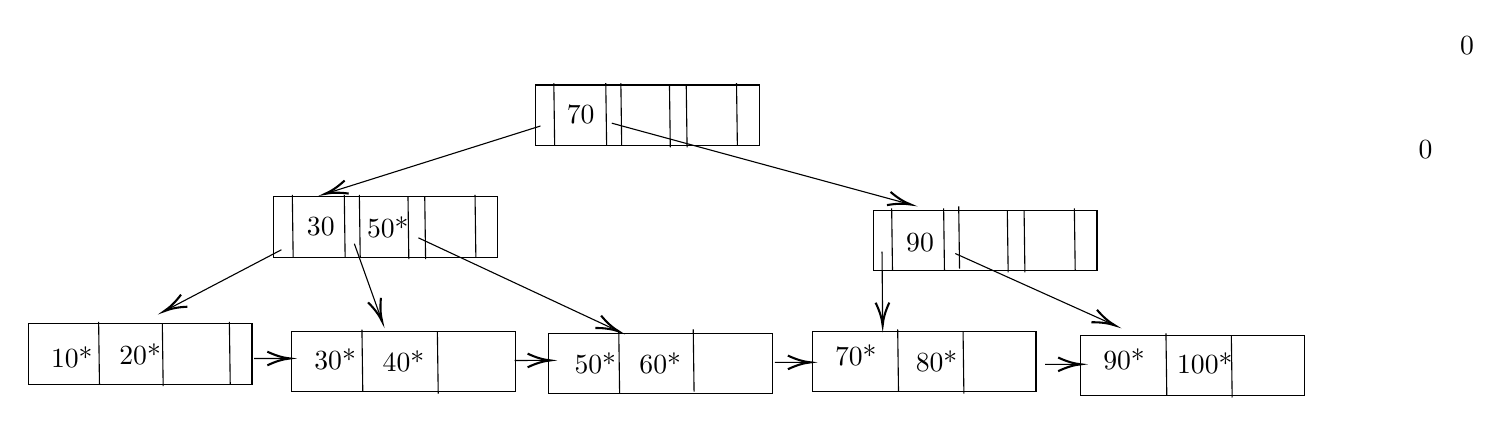
\begin{tikzpicture}[x=0.75pt,y=0.75pt,yscale=-1,xscale=1]
%uncomment if require: \path (0,345); %set diagram left start at 0, and has height of 345

%Shape: Rectangle [id:dp32574316465336217] 
\draw   (272.06,39.9) -- (379.88,39.9) -- (379.88,69.01) -- (272.06,69.01) -- cycle ;
%Straight Lines [id:da26653663223388] 
\draw    (305.98,39) -- (306.39,69.01) ;
%Straight Lines [id:da7385090454691864] 
\draw    (313.25,39) -- (313.65,69.01) ;
%Straight Lines [id:da8544299118360646] 
\draw    (280.95,39) -- (281.35,69.01) ;
%Straight Lines [id:da930732509680896] 
\draw    (336.67,39.9) -- (337.07,69.9) ;
%Straight Lines [id:da69512074796696] 
\draw    (344.75,39.9) -- (345.15,69.9) ;
%Straight Lines [id:da11381375915778624] 
\draw    (368.97,39) -- (369.38,69.01) ;
%Shape: Rectangle [id:dp5564235763237072] 
\draw   (146.08,93.74) -- (253.89,93.74) -- (253.89,122.85) -- (146.08,122.85) -- cycle ;
%Straight Lines [id:da102373038106776] 
\draw    (180,92.84) -- (180.4,122.85) ;
%Straight Lines [id:da5333943980458339] 
\draw    (187.26,92.84) -- (187.67,122.85) ;
%Straight Lines [id:da4097691419968579] 
\draw    (154.96,92.84) -- (155.36,122.85) ;
%Straight Lines [id:da3996471452585759] 
\draw    (210.69,93.74) -- (211.09,123.75) ;
%Straight Lines [id:da011032150201289226] 
\draw    (218.76,93.74) -- (219.17,123.75) ;
%Straight Lines [id:da802407879380034] 
\draw    (242.99,92.84) -- (243.39,122.85) ;
%Shape: Rectangle [id:dp9979129201079927] 
\draw   (434.84,100.18) -- (542.65,100.18) -- (542.65,129.29) -- (434.84,129.29) -- cycle ;
%Straight Lines [id:da16625765432954998] 
\draw    (468.76,99.29) -- (469.16,129.29) ;
%Straight Lines [id:da3647031842982146] 
\draw    (476.02,98.39) -- (476.43,128.4) ;
%Straight Lines [id:da8115786020974805] 
\draw    (443.72,99.29) -- (444.12,129.29) ;
%Straight Lines [id:da5222139177284297] 
\draw    (499.44,100.18) -- (499.85,130.19) ;
%Straight Lines [id:da24030239615721194] 
\draw    (507.52,100.18) -- (507.92,130.19) ;
%Straight Lines [id:da21971037892600864] 
\draw    (531.75,99.29) -- (532.15,129.29) ;
%Shape: Rectangle [id:dp13852793009269737] 
\draw   (27.72,154.93) -- (135.54,154.93) -- (135.54,184.03) -- (27.72,184.03) -- cycle ;
%Straight Lines [id:da5103414588651092] 
\draw    (61.64,154.03) -- (62.04,184.03) ;
%Straight Lines [id:da15205331219254947] 
\draw    (92.33,154.93) -- (92.73,184.93) ;
%Straight Lines [id:da7712823745198085] 
\draw    (124.63,154.03) -- (125.04,184.03) ;
%Shape: Rectangle [id:dp13870733259165058] 
\draw   (154.58,158.6) -- (262.4,158.6) -- (262.4,187.7) -- (154.58,187.7) -- cycle ;
%Straight Lines [id:da005178574681245163] 
\draw    (188.5,157.7) -- (188.91,187.7) ;
%Straight Lines [id:da7805076775703609] 
\draw    (224.84,158.6) -- (225.25,188.6) ;
%Shape: Rectangle [id:dp6253699450090605] 
\draw   (278.33,159.49) -- (386.14,159.49) -- (386.14,188.6) -- (278.33,188.6) -- cycle ;
%Straight Lines [id:da3239451920625164] 
\draw    (312.24,158.6) -- (312.65,188.6) ;
%Straight Lines [id:da6284444300247394] 
\draw    (348.12,157.62) -- (348.52,187.62) ;
%Shape: Rectangle [id:dp6137515015342755] 
\draw   (405.43,158.56) -- (513.25,158.56) -- (513.25,187.66) -- (405.43,187.66) -- cycle ;
%Straight Lines [id:da6413034625859316] 
\draw    (446.62,157.66) -- (447.02,187.66) ;
%Straight Lines [id:da5906079850634157] 
\draw    (478.12,158.56) -- (478.52,188.56) ;
%Straight Lines [id:da966696285693353] 
\draw    (274.49,59.64) -- (172.62,91.74) ;
\draw [shift={(170.71,92.34)}, rotate = 342.51] [color={rgb, 255:red, 0; green, 0; blue, 0 }  ][line width=0.75]    (10.93,-3.29) .. controls (6.95,-1.4) and (3.31,-0.3) .. (0,0) .. controls (3.31,0.3) and (6.95,1.4) .. (10.93,3.29)   ;
%Straight Lines [id:da5778572638983835] 
\draw    (308.87,58.27) -- (450.94,96.93) ;
\draw [shift={(452.87,97.45)}, rotate = 195.22] [color={rgb, 255:red, 0; green, 0; blue, 0 }  ][line width=0.75]    (10.93,-3.29) .. controls (6.95,-1.4) and (3.31,-0.3) .. (0,0) .. controls (3.31,0.3) and (6.95,1.4) .. (10.93,3.29)   ;
%Straight Lines [id:da6373025984910785] 
\draw    (149.71,119.26) -- (94.95,147.95) ;
\draw [shift={(93.18,148.87)}, rotate = 332.35] [color={rgb, 255:red, 0; green, 0; blue, 0 }  ][line width=0.75]    (10.93,-3.29) .. controls (6.95,-1.4) and (3.31,-0.3) .. (0,0) .. controls (3.31,0.3) and (6.95,1.4) .. (10.93,3.29)   ;
%Straight Lines [id:da5921462612949191] 
\draw    (184.84,116.34) -- (197.56,151.93) ;
\draw [shift={(198.24,153.81)}, rotate = 250.32999999999998] [color={rgb, 255:red, 0; green, 0; blue, 0 }  ][line width=0.75]    (10.93,-3.29) .. controls (6.95,-1.4) and (3.31,-0.3) .. (0,0) .. controls (3.31,0.3) and (6.95,1.4) .. (10.93,3.29)   ;
%Straight Lines [id:da9175068686245734] 
\draw    (215.71,113.52) -- (310.43,157.75) ;
\draw [shift={(312.24,158.6)}, rotate = 205.03] [color={rgb, 255:red, 0; green, 0; blue, 0 }  ][line width=0.75]    (10.93,-3.29) .. controls (6.95,-1.4) and (3.31,-0.3) .. (0,0) .. controls (3.31,0.3) and (6.95,1.4) .. (10.93,3.29)   ;
%Straight Lines [id:da5726521456220759] 
\draw    (136.61,171.66) -- (151.87,171.64) ;
\draw [shift={(153.87,171.63)}, rotate = 539.89] [color={rgb, 255:red, 0; green, 0; blue, 0 }  ][line width=0.75]    (10.93,-3.29) .. controls (6.95,-1.4) and (3.31,-0.3) .. (0,0) .. controls (3.31,0.3) and (6.95,1.4) .. (10.93,3.29)   ;
%Straight Lines [id:da40868810344831197] 
\draw    (262.01,172.6) -- (277.26,172.57) ;
\draw [shift={(279.26,172.57)}, rotate = 539.89] [color={rgb, 255:red, 0; green, 0; blue, 0 }  ][line width=0.75]    (10.93,-3.29) .. controls (6.95,-1.4) and (3.31,-0.3) .. (0,0) .. controls (3.31,0.3) and (6.95,1.4) .. (10.93,3.29)   ;
%Shape: Rectangle [id:dp5036188374691785] 
\draw   (534.69,160.43) -- (642.5,160.43) -- (642.5,189.54) -- (534.69,189.54) -- cycle ;
%Straight Lines [id:da9145477391462339] 
\draw    (575.87,159.53) -- (576.28,189.54) ;
%Straight Lines [id:da3181424664120508] 
\draw    (607.37,160.43) -- (607.77,190.44) ;
%Straight Lines [id:da531564246037878] 
\draw    (439.08,120.2) -- (439.36,153.69) ;
\draw [shift={(439.38,155.69)}, rotate = 269.52] [color={rgb, 255:red, 0; green, 0; blue, 0 }  ][line width=0.75]    (10.93,-3.29) .. controls (6.95,-1.4) and (3.31,-0.3) .. (0,0) .. controls (3.31,0.3) and (6.95,1.4) .. (10.93,3.29)   ;
%Straight Lines [id:da22139374645094956] 
\draw    (474.37,121.08) -- (549.45,154.87) ;
\draw [shift={(551.27,155.69)}, rotate = 204.23] [color={rgb, 255:red, 0; green, 0; blue, 0 }  ][line width=0.75]    (10.93,-3.29) .. controls (6.95,-1.4) and (3.31,-0.3) .. (0,0) .. controls (3.31,0.3) and (6.95,1.4) .. (10.93,3.29)   ;
%Straight Lines [id:da29975015663756754] 
\draw    (517.62,174.48) -- (532.87,174.45) ;
\draw [shift={(534.87,174.44)}, rotate = 539.89] [color={rgb, 255:red, 0; green, 0; blue, 0 }  ][line width=0.75]    (10.93,-3.29) .. controls (6.95,-1.4) and (3.31,-0.3) .. (0,0) .. controls (3.31,0.3) and (6.95,1.4) .. (10.93,3.29)   ;
%Straight Lines [id:da21491421802589095] 
\draw    (387.4,173.54) -- (402.66,173.51) ;
\draw [shift={(404.66,173.51)}, rotate = 539.89] [color={rgb, 255:red, 0; green, 0; blue, 0 }  ][line width=0.75]    (10.93,-3.29) .. controls (6.95,-1.4) and (3.31,-0.3) .. (0,0) .. controls (3.31,0.3) and (6.95,1.4) .. (10.93,3.29)   ;

% Text Node
\draw (721,21) node    {$0$};
% Text Node
\draw (701,71) node    {$0$};
% Text Node
\draw (293.87,54.26) node   [align=left] {70};
% Text Node
\draw (168.69,108.1) node   [align=left] {30};
% Text Node
\draw (48.72,171.08) node   [align=left] {10*};
% Text Node
\draw (175.58,172.06) node   [align=left] {30*};
% Text Node
\draw (300.94,173.85) node   [align=left] {50*};
% Text Node
\draw (426.43,170.22) node   [align=left] {70*};
% Text Node
\draw (457.41,115.91) node   [align=left] {90};
% Text Node
\draw (200.95,108.3) node   [align=left] {50*};
% Text Node
\draw (81.63,169.48) node   [align=left] {20*};
% Text Node
\draw (208.49,173.15) node   [align=left] {40*};
% Text Node
\draw (332.23,174.05) node   [align=left] {60*};
% Text Node
\draw (555.68,172.1) node   [align=left] {90*};
% Text Node
\draw (465.34,173.11) node   [align=left] {80*};
% Text Node
\draw (594.6,174.05) node   [align=left] {100*};


\end{tikzpicture}


\end{itemize}
\part{3} 
\begin{itemize}
\item[(a)] 


\tikzset{every picture/.style={line width=0.75pt}} %set default line width to 0.75pt        

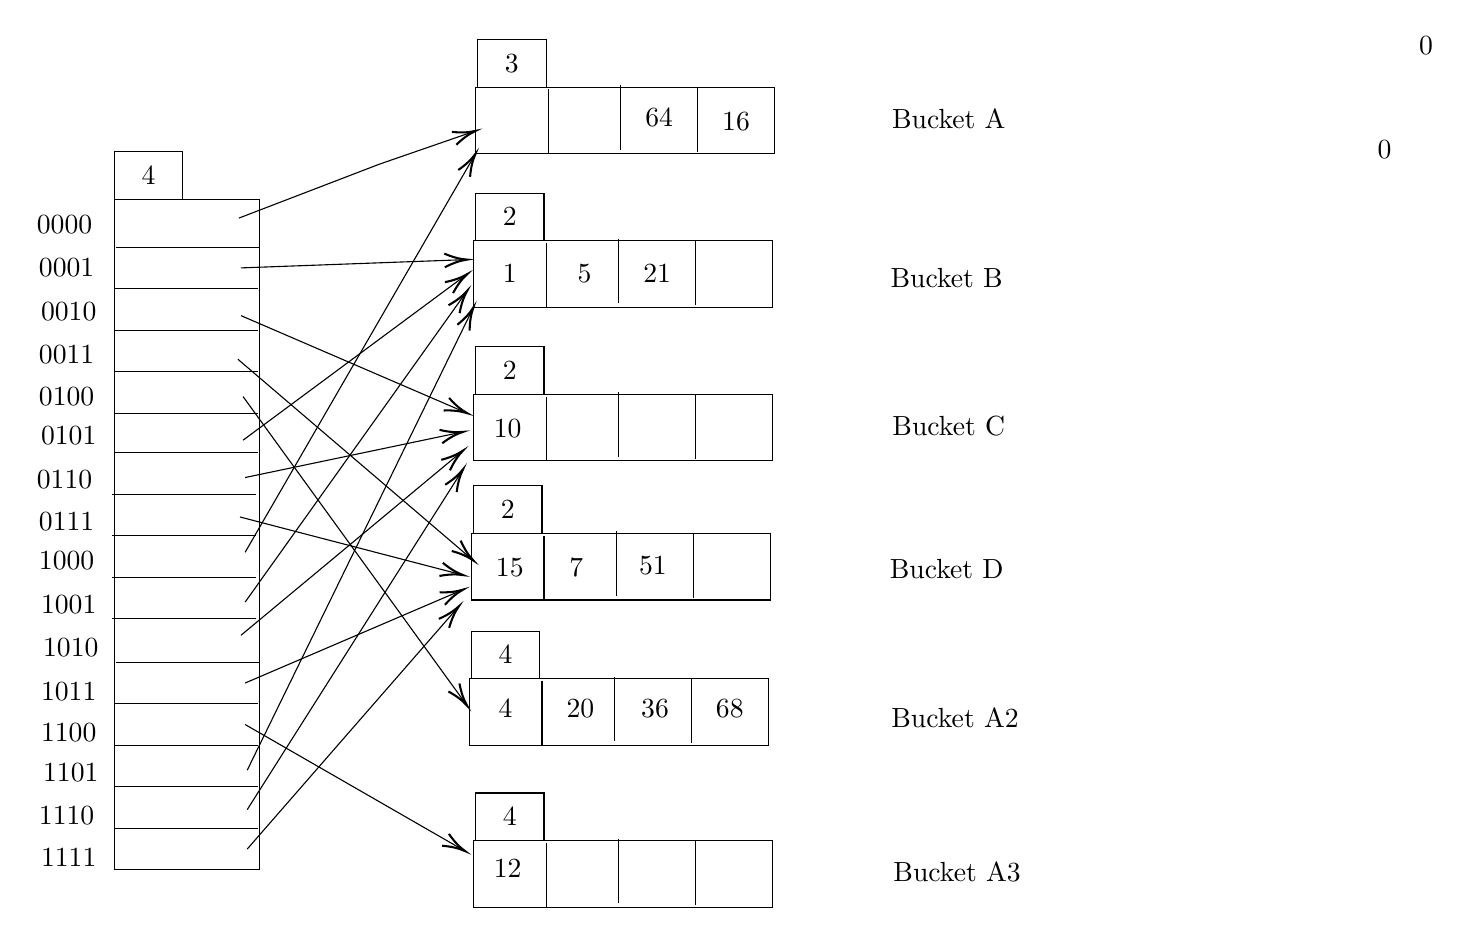
\begin{tikzpicture}[x=0.75pt,y=0.75pt,yscale=-1,xscale=1]
%uncomment if require: \path (0,597); %set diagram left start at 0, and has height of 597

%Shape: Rectangle [id:dp5088674491093252] 
\draw   (89,95) -- (159,95) -- (159,418) -- (89,418) -- cycle ;
%Straight Lines [id:da38815688020973005] 
\draw    (90,118) -- (159,118) ;
%Straight Lines [id:da29283758864363985] 
\draw    (89,138) -- (158,138) ;
%Straight Lines [id:da8254093647387246] 
\draw    (89,158) -- (158,158) ;
%Straight Lines [id:da2169244859202757] 
\draw    (89,178) -- (158,178) ;
%Straight Lines [id:da7128070968298222] 
\draw    (89,198) -- (158,198) ;
%Straight Lines [id:da4495119983149207] 
\draw    (89,217) -- (158,217) ;
%Straight Lines [id:da7729270157734506] 
\draw    (88,237) -- (157,237) ;
%Straight Lines [id:da27170025620254135] 
\draw    (88,257) -- (157,257) ;
%Straight Lines [id:da25267888366641134] 
\draw    (88,277) -- (157,277) ;
%Straight Lines [id:da08312820896301631] 
\draw    (88,297) -- (157,297) ;
%Straight Lines [id:da658684501684739] 
\draw    (90,318) -- (159,318) ;
%Straight Lines [id:da46434505993319763] 
\draw    (89,338) -- (158,338) ;
%Straight Lines [id:da019589634465967953] 
\draw    (89,358) -- (158,358) ;
%Straight Lines [id:da9115822403212651] 
\draw    (89,378) -- (158,378) ;
%Straight Lines [id:da9091752806311868] 
\draw    (89,398) -- (158,398) ;
%Shape: Rectangle [id:dp2567182952120206] 
\draw   (263,41) -- (407,41) -- (407,73) -- (263,73) -- cycle ;
%Shape: Rectangle [id:dp152344519607428] 
\draw   (89,72) -- (122,72) -- (122,95) -- (89,95) -- cycle ;
%Straight Lines [id:da9190809179671136] 
\draw    (298,42) -- (298,73) ;
%Straight Lines [id:da7189894952172353] 
\draw    (333,40) -- (333,71) ;
%Straight Lines [id:da3567981472782338] 
\draw    (370,41) -- (370,72) ;
%Shape: Rectangle [id:dp14201576149636652] 
\draw   (264,18) -- (297,18) -- (297,41) -- (264,41) -- cycle ;
%Shape: Rectangle [id:dp7106384652403785] 
\draw   (262,115) -- (406,115) -- (406,147) -- (262,147) -- cycle ;
%Straight Lines [id:da9503665327369227] 
\draw    (297,116) -- (297,147) ;
%Straight Lines [id:da5737916321075605] 
\draw    (332,114) -- (332,145) ;
%Straight Lines [id:da9994783907024051] 
\draw    (369,115) -- (369,146) ;
%Shape: Rectangle [id:dp3509013459169691] 
\draw   (263,92) -- (296,92) -- (296,115) -- (263,115) -- cycle ;
%Shape: Rectangle [id:dp8041479329735063] 
\draw   (262,189) -- (406,189) -- (406,221) -- (262,221) -- cycle ;
%Straight Lines [id:da8971360172254296] 
\draw    (297,190) -- (297,221) ;
%Straight Lines [id:da9907834600017352] 
\draw    (332,188) -- (332,219) ;
%Straight Lines [id:da9011603529452705] 
\draw    (369,189) -- (369,220) ;
%Shape: Rectangle [id:dp2804376702207778] 
\draw   (263,166) -- (296,166) -- (296,189) -- (263,189) -- cycle ;
%Shape: Rectangle [id:dp609401588414675] 
\draw   (261,256) -- (405,256) -- (405,288) -- (261,288) -- cycle ;
%Straight Lines [id:da29579569701994457] 
\draw    (296,257) -- (296,288) ;
%Straight Lines [id:da8310522676226318] 
\draw    (331,255) -- (331,286) ;
%Straight Lines [id:da7523517919512148] 
\draw    (368,256) -- (368,287) ;
%Shape: Rectangle [id:dp7438419177045621] 
\draw   (262,233) -- (295,233) -- (295,256) -- (262,256) -- cycle ;
%Shape: Rectangle [id:dp12392268230040338] 
\draw   (260,326) -- (404,326) -- (404,358) -- (260,358) -- cycle ;
%Straight Lines [id:da5806856268991099] 
\draw    (295,327) -- (295,358) ;
%Straight Lines [id:da22950329852341067] 
\draw    (330,325) -- (330,356) ;
%Straight Lines [id:da5575859603980332] 
\draw    (367,326) -- (367,357) ;
%Shape: Rectangle [id:dp9647701583904539] 
\draw   (261,303) -- (294,303) -- (294,326) -- (261,326) -- cycle ;
%Shape: Rectangle [id:dp7704590305825274] 
\draw   (262,404) -- (406,404) -- (406,436) -- (262,436) -- cycle ;
%Straight Lines [id:da04605926112607528] 
\draw    (297,405) -- (297,436) ;
%Straight Lines [id:da007576995713324597] 
\draw    (332,403) -- (332,434) ;
%Straight Lines [id:da03706328294855954] 
\draw    (369,404) -- (369,435) ;
%Shape: Rectangle [id:dp19750166184952922] 
\draw   (263,381) -- (296,381) -- (296,404) -- (263,404) -- cycle ;
%Straight Lines [id:da16018695078795675] 
\draw    (149,104) -- (216.66,78.03) -- (261.11,62.65) ;
\draw [shift={(263,62)}, rotate = 520.9200000000001] [color={rgb, 255:red, 0; green, 0; blue, 0 }  ][line width=0.75]    (10.93,-3.29) .. controls (6.95,-1.4) and (3.31,-0.3) .. (0,0) .. controls (3.31,0.3) and (6.95,1.4) .. (10.93,3.29)   ;
%Straight Lines [id:da9985415872475967] 
\draw    (150,128) -- (257,124.07) ;
\draw [shift={(259,124)}, rotate = 537.9] [color={rgb, 255:red, 0; green, 0; blue, 0 }  ][line width=0.75]    (10.93,-3.29) .. controls (6.95,-1.4) and (3.31,-0.3) .. (0,0) .. controls (3.31,0.3) and (6.95,1.4) .. (10.93,3.29)   ;
%Straight Lines [id:da15036524887808644] 
\draw    (150,151) -- (257.16,197.21) ;
\draw [shift={(259,198)}, rotate = 203.32999999999998] [color={rgb, 255:red, 0; green, 0; blue, 0 }  ][line width=0.75]    (10.93,-3.29) .. controls (6.95,-1.4) and (3.31,-0.3) .. (0,0) .. controls (3.31,0.3) and (6.95,1.4) .. (10.93,3.29)   ;
%Straight Lines [id:da1385508019867896] 
\draw    (148.5,172) -- (260.48,267.7) ;
\draw [shift={(262,269)}, rotate = 220.52] [color={rgb, 255:red, 0; green, 0; blue, 0 }  ][line width=0.75]    (10.93,-3.29) .. controls (6.95,-1.4) and (3.31,-0.3) .. (0,0) .. controls (3.31,0.3) and (6.95,1.4) .. (10.93,3.29)   ;
%Straight Lines [id:da7770813038411519] 
\draw    (151,190) -- (257.83,337.38) ;
\draw [shift={(259,339)}, rotate = 234.06] [color={rgb, 255:red, 0; green, 0; blue, 0 }  ][line width=0.75]    (10.93,-3.29) .. controls (6.95,-1.4) and (3.31,-0.3) .. (0,0) .. controls (3.31,0.3) and (6.95,1.4) .. (10.93,3.29)   ;
%Straight Lines [id:da27643105330197726] 
\draw    (151,211) -- (257.39,132.19) ;
\draw [shift={(259,131)}, rotate = 503.47] [color={rgb, 255:red, 0; green, 0; blue, 0 }  ][line width=0.75]    (10.93,-3.29) .. controls (6.95,-1.4) and (3.31,-0.3) .. (0,0) .. controls (3.31,0.3) and (6.95,1.4) .. (10.93,3.29)   ;
%Straight Lines [id:da8085280275571725] 
\draw    (152,229) -- (255.04,207.41) ;
\draw [shift={(257,207)}, rotate = 528.1700000000001] [color={rgb, 255:red, 0; green, 0; blue, 0 }  ][line width=0.75]    (10.93,-3.29) .. controls (6.95,-1.4) and (3.31,-0.3) .. (0,0) .. controls (3.31,0.3) and (6.95,1.4) .. (10.93,3.29)   ;
%Straight Lines [id:da09719931405883409] 
\draw    (149.5,248) -- (255.06,275.5) ;
\draw [shift={(257,276)}, rotate = 194.6] [color={rgb, 255:red, 0; green, 0; blue, 0 }  ][line width=0.75]    (10.93,-3.29) .. controls (6.95,-1.4) and (3.31,-0.3) .. (0,0) .. controls (3.31,0.3) and (6.95,1.4) .. (10.93,3.29)   ;
%Straight Lines [id:da6830224749759807] 
\draw    (152,265) -- (262,74.73) ;
\draw [shift={(263,73)}, rotate = 480.03] [color={rgb, 255:red, 0; green, 0; blue, 0 }  ][line width=0.75]    (10.93,-3.29) .. controls (6.95,-1.4) and (3.31,-0.3) .. (0,0) .. controls (3.31,0.3) and (6.95,1.4) .. (10.93,3.29)   ;
%Straight Lines [id:da0946614699937689] 
\draw    (152,289) -- (257.84,140.63) ;
\draw [shift={(259,139)}, rotate = 485.5] [color={rgb, 255:red, 0; green, 0; blue, 0 }  ][line width=0.75]    (10.93,-3.29) .. controls (6.95,-1.4) and (3.31,-0.3) .. (0,0) .. controls (3.31,0.3) and (6.95,1.4) .. (10.93,3.29)   ;
%Straight Lines [id:da08998871529335473] 
\draw    (150,305) -- (255.46,217.28) ;
\draw [shift={(257,216)}, rotate = 500.25] [color={rgb, 255:red, 0; green, 0; blue, 0 }  ][line width=0.75]    (10.93,-3.29) .. controls (6.95,-1.4) and (3.31,-0.3) .. (0,0) .. controls (3.31,0.3) and (6.95,1.4) .. (10.93,3.29)   ;
%Straight Lines [id:da435578731886727] 
\draw    (152,328) -- (255.16,283.79) ;
\draw [shift={(257,283)}, rotate = 516.8] [color={rgb, 255:red, 0; green, 0; blue, 0 }  ][line width=0.75]    (10.93,-3.29) .. controls (6.95,-1.4) and (3.31,-0.3) .. (0,0) .. controls (3.31,0.3) and (6.95,1.4) .. (10.93,3.29)   ;
%Straight Lines [id:da013534431457925322] 
\draw    (152,348) -- (256.27,408) ;
\draw [shift={(258,409)}, rotate = 209.92000000000002] [color={rgb, 255:red, 0; green, 0; blue, 0 }  ][line width=0.75]    (10.93,-3.29) .. controls (6.95,-1.4) and (3.31,-0.3) .. (0,0) .. controls (3.31,0.3) and (6.95,1.4) .. (10.93,3.29)   ;
%Straight Lines [id:da5369784630867279] 
\draw    (153,370) -- (261.12,148.8) ;
\draw [shift={(262,147)}, rotate = 476.05] [color={rgb, 255:red, 0; green, 0; blue, 0 }  ][line width=0.75]    (10.93,-3.29) .. controls (6.95,-1.4) and (3.31,-0.3) .. (0,0) .. controls (3.31,0.3) and (6.95,1.4) .. (10.93,3.29)   ;
%Straight Lines [id:da8476280502250436] 
\draw    (153,389) -- (255.93,226.69) ;
\draw [shift={(257,225)}, rotate = 482.38] [color={rgb, 255:red, 0; green, 0; blue, 0 }  ][line width=0.75]    (10.93,-3.29) .. controls (6.95,-1.4) and (3.31,-0.3) .. (0,0) .. controls (3.31,0.3) and (6.95,1.4) .. (10.93,3.29)   ;
%Straight Lines [id:da9110406512913233] 
\draw    (153,408) -- (253.69,292.51) ;
\draw [shift={(255,291)}, rotate = 491.08] [color={rgb, 255:red, 0; green, 0; blue, 0 }  ][line width=0.75]    (10.93,-3.29) .. controls (6.95,-1.4) and (3.31,-0.3) .. (0,0) .. controls (3.31,0.3) and (6.95,1.4) .. (10.93,3.29)   ;

% Text Node
\draw (721,21) node    {$0$};
% Text Node
\draw (701,71) node    {$0$};
% Text Node
\draw (65,107) node   [align=left] {0000};
% Text Node
\draw (66,128) node   [align=left] {0001};
% Text Node
\draw (67,149) node   [align=left] {0010};
% Text Node
\draw (66,170) node   [align=left] {0011};
% Text Node
\draw (66,190) node   [align=left] {0100};
% Text Node
\draw (67,209) node   [align=left] {0101};
% Text Node
\draw (65,230) node   [align=left] {0110};
% Text Node
\draw (66,250) node   [align=left] {0111};
% Text Node
\draw (66,269) node   [align=left] {1000};
% Text Node
\draw (67,290) node   [align=left] {1001};
% Text Node
\draw (68,311) node   [align=left] {1010};
% Text Node
\draw (67,332) node   [align=left] {1011};
% Text Node
\draw (67,352) node   [align=left] {1100};
% Text Node
\draw (68,371) node   [align=left] {1101};
% Text Node
\draw (66,392) node   [align=left] {1110};
% Text Node
\draw (67,412) node   [align=left] {1111};
% Text Node
\draw (105.5,83.5) node   [align=left] {4};
% Text Node
\draw (280.5,29.5) node   [align=left] {3};
% Text Node
\draw (279.5,103.5) node   [align=left] {2};
% Text Node
\draw (279.5,177.5) node   [align=left] {2};
% Text Node
\draw (278.5,244.5) node   [align=left] {2};
% Text Node
\draw (277.5,314.5) node   [align=left] {4};
% Text Node
\draw (279.5,392.5) node   [align=left] {4};
% Text Node
\draw (491,56) node   [align=left] {Bucket A};
% Text Node
\draw (490,133) node   [align=left] {Bucket B};
% Text Node
\draw (491,204) node   [align=left] {Bucket C};
% Text Node
\draw (490,273) node   [align=left] {Bucket D};
% Text Node
\draw (494,345) node   [align=left] {Bucket A2};
% Text Node
\draw (495,419) node   [align=left] {Bucket A3};
% Text Node
\draw (351.5,55.5) node   [align=left] {64};
% Text Node
\draw (388.5,57.5) node   [align=left] {16};
% Text Node
\draw (278.5,417.5) node   [align=left] {12};
% Text Node
\draw (277.5,340.5) node   [align=left] {4};
% Text Node
\draw (313.5,340.5) node   [align=left] {20};
% Text Node
\draw (349.5,340.5) node   [align=left] {36};
% Text Node
\draw (385.5,340.5) node   [align=left] {68};
% Text Node
\draw (279.5,272.5) node   [align=left] {15};
% Text Node
\draw (311.5,272.5) node   [align=left] {7};
% Text Node
\draw (348.5,271.5) node   [align=left] {51};
% Text Node
\draw (278.5,205.5) node   [align=left] {10};
% Text Node
\draw (279.5,130.5) node   [align=left] {1};
% Text Node
\draw (315.5,130.5) node   [align=left] {5};
% Text Node
\draw (350.5,130.5) node   [align=left] {21};
\end{tikzpicture}

\item[(b)]  The minimal set of deletion to trigger a merge is $\{64, 16 \}$. That is, when this set is deleted, there can be a merge between bucket A and A2. One might think that the answer should be $\{10 \}$, but, in this case, the bucket C is already a primary page and it has to be left as a place holder. 
\end{itemize}

\question{Exam Revisit}{}
\part{1} Set-model will not give the right answer in querying for the average score of a class. This is because set model will contain no duplicates and the exam scores are not guaranteed to be unique. Therefore, Bag Model it is!

\part{2} 
\begin{verbatim}
SELECT DISTINCT maker FROM Computer WHERE model in(
SELECT model FROM PC WHERE speed in (
SELECT speed FROM PC ORDER BY  speed  DESC LIMIT 1);
\end{verbatim}

\part{3}    given $R(A,B,C,D)$ and $ \mathcal{F} =\{AC \rightarrow B, B \rightarrow A, BD \rightarrow C, D \rightarrow A \}$ Find the candidate keys.
\begin{itemize}
\item $BD \quad \because BD^+ = \{ A,B ,C, D\}$ 
\item $CD \quad \because CD^+ = \{ A,B ,C, D\}$ 
\end{itemize}


\part{4}  Basis and Minimal basis
\begin{itemize}
\item The right hand side of the dependency cannot contain more than one attribute to be a \textit{\textbf{minimal basis}} .
\item $\mathcal{G}$ is a \textit{\textbf{basis}} of $ \mathcal{F}$ and vice versa. This is because the two sets of dependencies are equivalent. 
\item $\mathcal{M} = \{ A \rightarrow B\, A \rightarrow C \}$ is a minimal basis of $\mathcal{F}$ since it meets the following three criteria:
\begin{itemize}
\item[(i)] All FDs in $\mathcal{M} $  have singleton right sides.
\item[(ii)] Any FD in $\mathcal{M} $  is removed, then the result is no longer a basis
\item[(iii)] For any FD in $\mathcal{M}$ we remove one or more attributes from the left side of F, the result is no longer a basis.
\end{itemize} 
\end{itemize}



\end{document}

